\documentclass[12pt, oneside]{article}
\usepackage[letterpaper, margin=1in, headsep=0.5in]{geometry}
\usepackage[english]{babel}
\usepackage[utf8]{inputenc}
\usepackage{amsmath}
\usepackage{amsfonts}
\usepackage{amssymb}
\usepackage{tikz}
\usepackage{tkz-fct}
\usepackage{pgfplots}
\pgfplotsset{width=10cm,compat=1.9}
\usepgfplotslibrary{statistics}
\usepackage{pgfplotstable}
%\usepackage{venndiagram}

\usepackage{fancyhdr}
\pagestyle{fancy}
\fancyhf{}
\rhead{\thepage \\Name: \hspace{1.5in}.\\}
\lhead{BECA / Dr. Huson / 11.2 Algebra 2\\* 9 May 2018 \\*\textbf{Classwork: Pretest polynomial functions
}}

\renewcommand{\headrulewidth}{0pt}

\begin{document}


%\subsection*{Solve equations}

%Solve for the value of $x$.
\vspace{1cm}

\begin{enumerate}

\item Determine whether the binomial $x+3$ is a factor of $f(x)=3x^3+10x^2-x-12$.\\[5in]

\item Given $r(x)=x^3-4x^2+4x-6$, find the value of $r(2)$.\\*[2in]
What does your answer tell you about $x-2$ as a factor of $r(x)$? Explain. %Alg2 Regents Jun2017 

\newpage
\item The graph of the function $p(x)$ is sketched below.
\begin{center}
    \begin{tikzpicture}[scale=2.54/4]
    \draw[thick,<->] (-4.5,0) -- (5.5,0) node[anchor=north west] {\textbf{x}};
    \draw[thick,<->] (0,-3.5) -- (0,7.5) node[anchor=south east] {\textbf{p(x)}};
    \foreach \x in {-1, 1} \draw (\x cm,5pt) -- (\x cm,-5pt) node[anchor=north] {$\x$};
    \foreach \x in {-4,-3,-2, 2, 3, 4} \draw (\x cm,5pt) -- (\x cm,-5pt) node[anchor=north] {};
    %\foreach \y in {5} \draw (1pt,\y cm) -- (-1pt,\y cm) node[anchor=east] {50}; %{$\y$};
    \tkzInit[xmin=-5,xmax=5,ymin=-7,ymax=7,ystep=1]   
    \tkzFct[color=black,very thick,<->,domain = -3.2:4] {0.2*(x*x-9)*(x-2)};
    \end{tikzpicture}
\end{center}
Which equation could represent $p(x)$?
\begin{enumerate}
    \item $p(x)=(x^2- 9)(x-2)$
    \item $p(x)=x^3 -2x^2+ 9x+18$
    \item $p(x)=(x^2+ 9)(x-2)$
    \item $p(x)=x^3 +2x^2- 9x-18$
\end{enumerate} %Alg2 Regents Jun2017 multiple choice

\item A manufacturing company has developed a cost model, $C(x)=0.15x^3+0.01x^2+2x+120$, where $x$ is the number of items sold, in thousands. The sales price can be modeled by $S(x)=30-0.01x$. Therefore, revenue is modeled by $R(x)=x \cdot S(x)$.\\*[5pt]
The company’s profit, $P(x)=R(x)-C(x)$, could be modeled by what polynomial?  %Alg2 Regents Jun2017 multiple choice

\newpage

\item A bank account earns interest at a continuous interest rate of 4\% per year. The initial deposit is \$175.
\begin{enumerate}
    \item Express the balance in the account as a function in the form $P(t)=P_0 \cdot e^{rt}$\\[30pt]
    \item Convert the function to one without a coefficient in the exponent. \\[30pt]
    \item What is the interest rate expressed as a simple, annual rate?\\[30pt]
\end{enumerate}

\item Judith puts \$2500 into an investment account with interest compounded continuously. If the annual interest rate is 2.15\% what is the balance after 20 years?\\[80pt]

\item The function below models the average price of gas in a small town since January 1st.
\[G(t)=0.0812t^3 - 0.75t^2 +1.25t+3.23 \text{, where } 0 \leq t \leq 5.\]
If $G(t)$ is the average price of gas in dollars and $t$ represents the number of months since January 1st, the absolute maximum $G(t)$ reaches over the given domain is about what value, to the nearest cent? (graph the function in your calculator and use the Max function)%Alg2 Regents Jan2018

\newpage


\item Write $\sqrt[3]x^5$ as a single term with a rational exponent.\\*[30pt]

\item Write $\sqrt{a^4} \div a^{\frac{1}{2}}$ as an expression with positive, integer exponents.\\*[30pt]

\item If $n=\sqrt{z^3}$ and $m=z$, where $a > 0$, express $\frac{n}{m}$ as 
\begin{enumerate}
    \item a radical with positive, integer exponents\\*[30pt]
    \item an expression with a fractional exponent\\*[30pt]
\end{enumerate}

\item What is the expression $2i^3(-3i+7)$ is equivalent to? Express your answer in the form $a+bi$, where $a, b \in \mathbb{R}$.\\*[30pt]  %Alg2 Regents Jun2017 multiple choice

\item Simplify the expression $(1x - 3i)^2$, where $i$ is the imaginary unit. Express your answer in the form $a+bi$, where $a, b \in \mathbb{R}$.\\[30pt] %Alg2 Regents Aug2017

\item Algebraically determine the values of $h$ and $k$ to correctly complete the identity stated below.
\[3x^3-7x^2+5x-5=(x-2)(3x^2+hx+k)\] %Alg2 Regents Jan 2017

\newpage
\item Graph the function $f(x)=x^3-3x^2+2$. 
\begin{enumerate}
    \item Write down the $y$-intercept.\\*[10pt]
    \item Mark the $x$-intercepts on the graph as ordered pairs, rounding to the nearest hundredth.\\*[10pt]
    \item Describe the end behavior of the function. (use language like "As $x$ goes to positive infinity, $y$ goes to...")\\*[50pt]
\end{enumerate}

\begin{figure}[!ht]
    \centering
    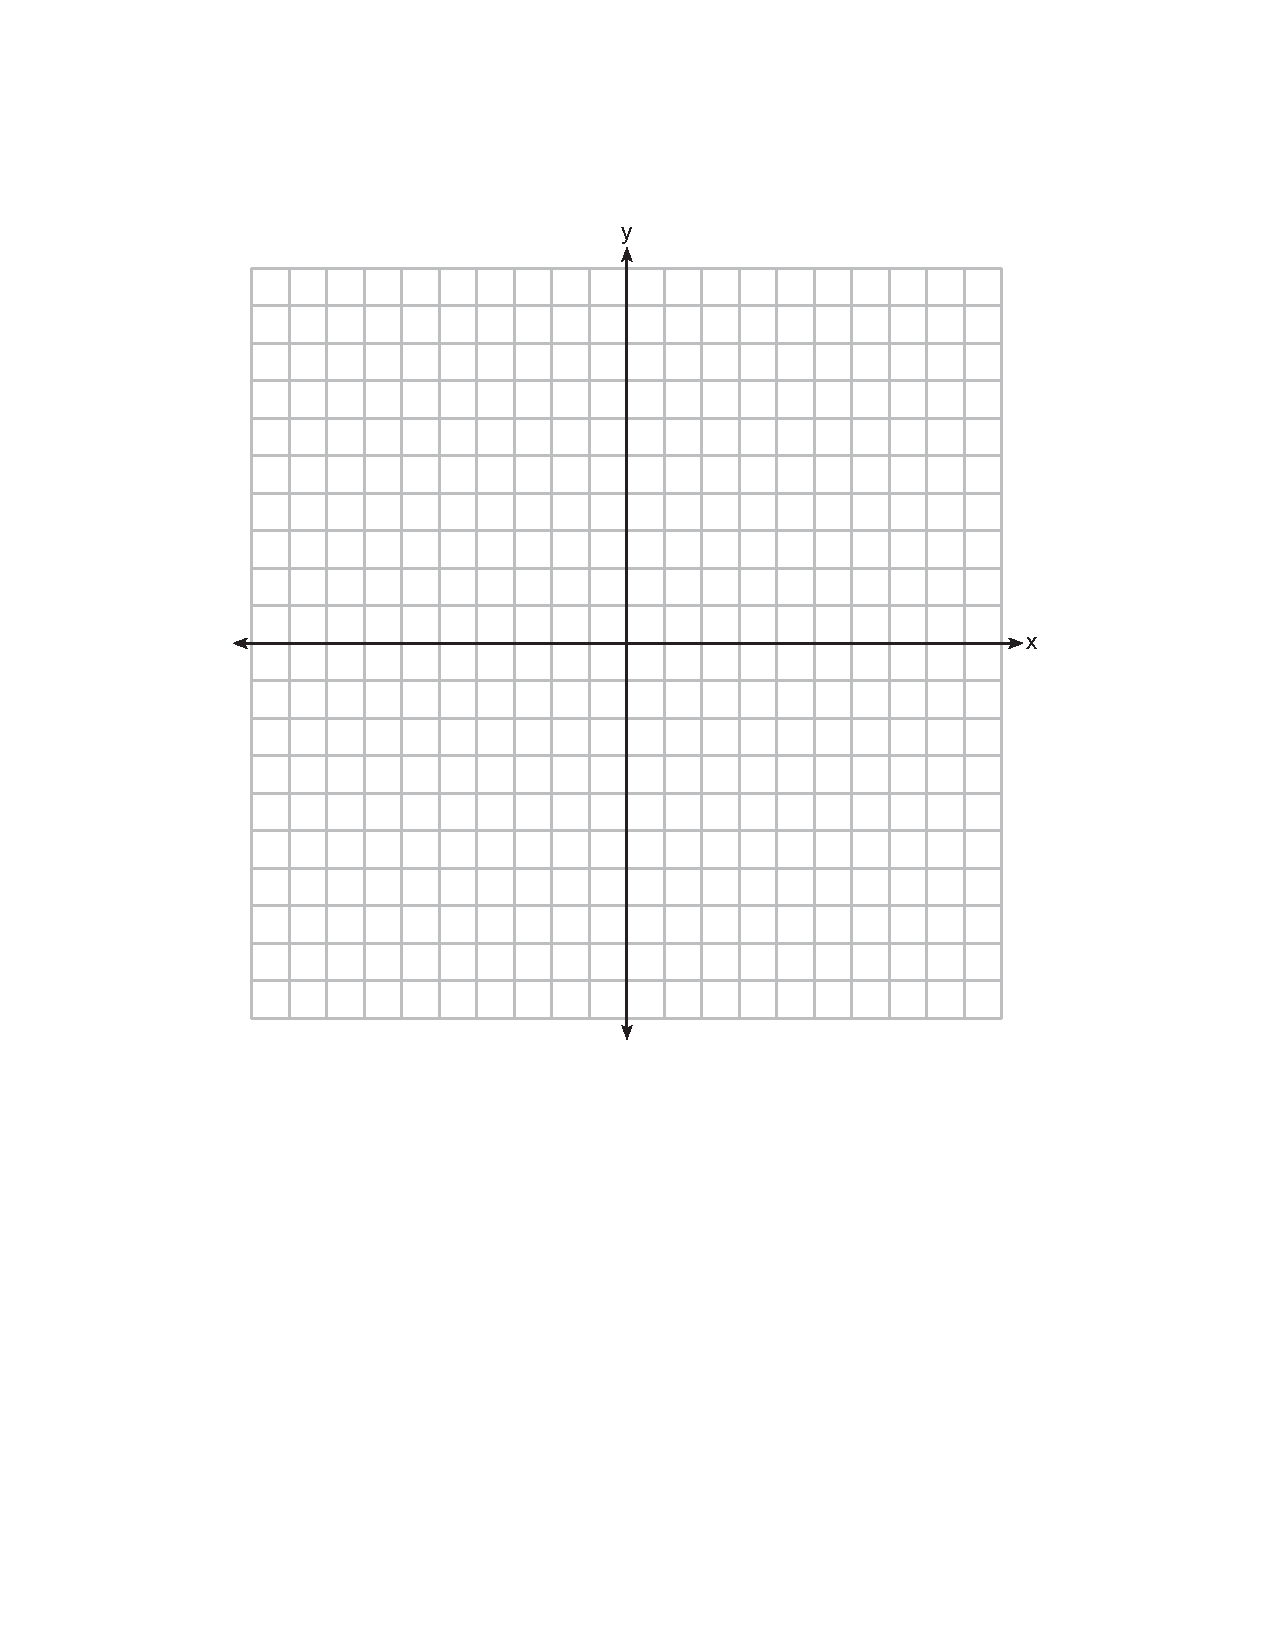
\includegraphics[width=0.75\textwidth]{regents-grid.pdf}
\end{figure}

\newpage
\item The expression $(x + a)(x + b)$ can not be written as
\begin{enumerate}
    \item $a(x + b)+ x(x + b)$
    \item $x^2 + (a - b)x + ab$ 
    \item  $x^2 + (a + b)x + ab$  
    \item $x(x + a)+ b(x + a)$
\end{enumerate}

\item What is the quotient and the remainder when $3x^3+8x^2+7x+3$ is divided by $x+2$?\\*[50pt]

\newpage
\item Judith puts \$1000 into an investment account with interest compounded continuously. What is the approximate annual rate is needed for the account to grow to \$1529.59 after 10 years?

\item The function $p(t)=110e^{0.03922t}$ models the population of a city, in millions, $t$ years after 2010.
\begin{enumerate}
    \item Initially, as of 2010, what is the population in millions.\\[40pt]
    \item What is the rate that the population increases continuously, per year?\\[40pt]
    \item Express the population as a function with the form $p(t)=Ab^{t}$, where $A$ and $b$ are real numbers.\\[40pt]
\end{enumerate}

\item For a given time, $x$, in seconds, an electric current, $y$, can be represented by $y = 2.7^{-.10x}$. 
\begin{enumerate}
    \item Simplify the expression to eliminate the coefficient in the exponent.\\[40pt]
    \item Is the electric current increasing or decreasing? Justify your answer.\\[70pt]
    \item Is the current in the original equation, above, exponential growth or decay? Why?\\[70pt]
\end{enumerate}

\newpage

\item Iridium-192 is an isotope of iridium and has a half-life of 73.83 days. If a laboratory experiment begins with 100 grams of Iridium-192, the number of grams, $A$, of Iridium-192 present after $t$ days would be 
\[A=100 \left( \frac{1}{2} \right)^\frac{t}{73.83}\]

\begin{enumerate}
    \item Simplify the equation to eliminate the fraction in the exponent.\\[30pt]
    \item After one day, how much isotope is present?\\[30pt]
    \item As a percentage, how much does the mass of the isotope change each day?\\[30pt]
\end{enumerate}


\end{enumerate}
\end{document}